\begin{frame}
    \frametitle{Cámara}
    
%    \includegraphics[width=0.4\columnwidth]{images/camera/}
%    \includegraphics[width=0.4\columnwidth]{images/camera/}
    \footnotesize
    
    \begin{block}{Principio de funcionamiento}
    	
    \end{block}

\end{frame}

\begin{frame}
	\frametitle{Distorción}
	
	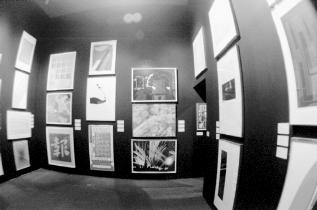
\includegraphics[width=0.4\columnwidth]{images/camera/distorted_image.png}
	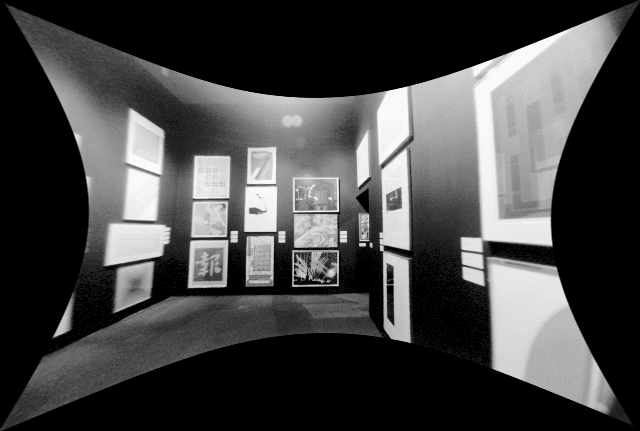
\includegraphics[width=0.4\columnwidth]{images/camera/undistorted_image.png}
	
\end{frame}


\begin{frame}
	\frametitle{Distorción}
	
	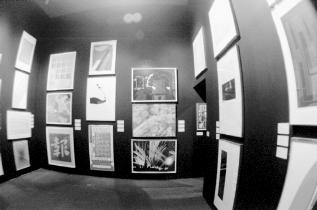
\includegraphics[width=0.4\columnwidth]{images/camera/distorted_image.png}
	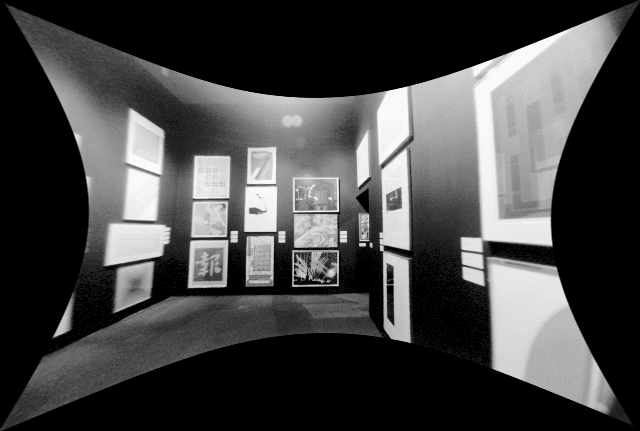
\includegraphics[width=0.4\columnwidth]{images/camera/undistorted_image.png}
	
\end{frame}


\begin{frame}
	\frametitle{Características Visuales: Detector FAST}
	
	\begin{figure}
		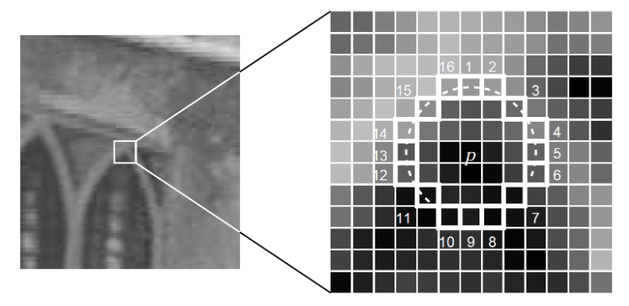
\includegraphics[width=0.8\textwidth]{./images/camera/fast}
	\end{figure}
	
	El valor de intensidad del pixel $p$ es comparado con cada uno de los 16 pixeles del círculo de Bresenham alrededor de $p$. $p$ es detectado como corner si hay $12$ píxeles continuos en el circulo de Bresenham más brillosos o oscuros que $p$ dado un cierto umbral.
\end{frame}

\begin{frame}
	\frametitle{Características Visuales: Descriptor BRIEF}
	\begin{minipage}[t]{0.35\columnwidth}
		\begin{figure}
			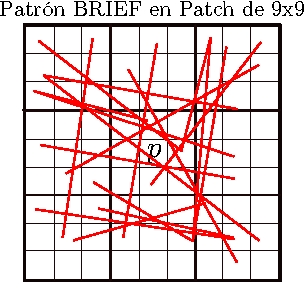
\includegraphics[width=\columnwidth]{./images/camera/brief}
		\end{figure}
	\end{minipage}\hfill{}
	\begin{minipage}[t]{0.6\columnwidth}
		\centering
		256 Comparaciones entre píxeles (1 a 1)
		\begin{equation*}
			\tau(p;x,y) =
			\begin{cases}
				1 & \text{if $p(x) < p(y)$}\\
				0 & \text{otherwise}\\
			\end{cases}     
		\end{equation*}
		$s = \overbrace{01010010101110010...}^{256\ \text{bits}}$
	\end{minipage}
	\begin{block}{Matching distance}
		$\text{Hamming distance} = sum (XOR(s_{1}, s_{2}))$
	\end{block}
	\note{utilizamos la distancia de hamming para la distancia de matcheo entre descriptores.}
\end{frame}
